
\section{Preliminaries}
\label{sec:Preliminaries}

\begin{figure*}[!ht]
\centering
    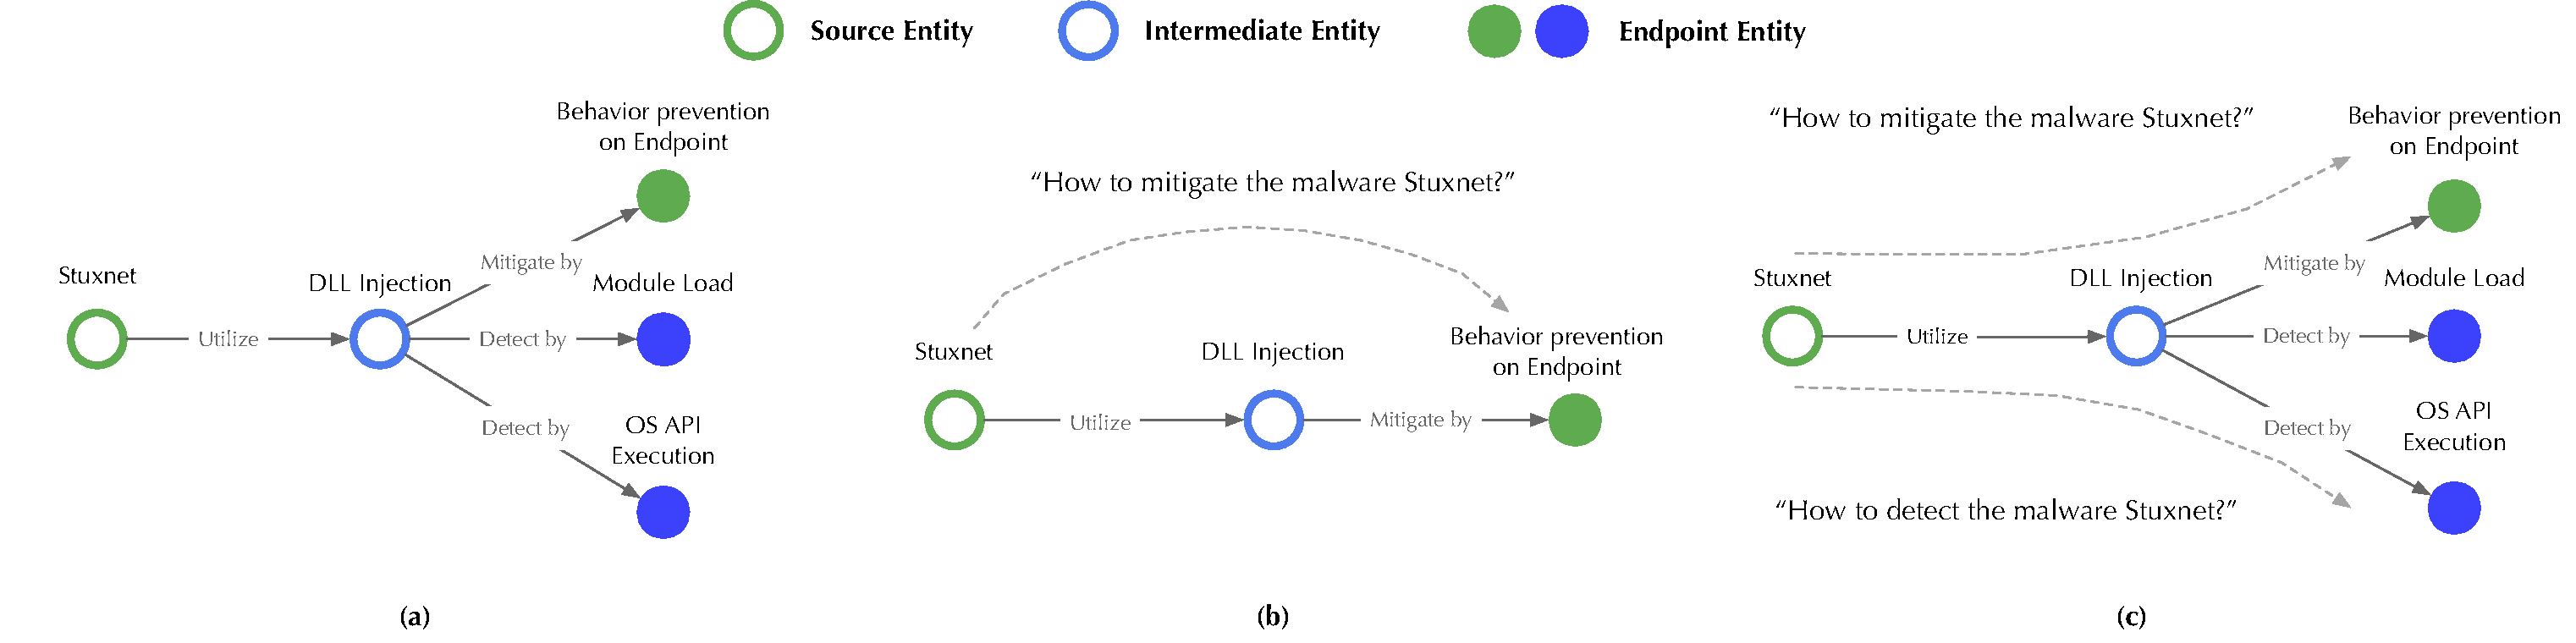
\includegraphics[width=\linewidth]{figs_false/fg2.pdf}
% \subfloat[]{\includegraphics[width=2in]{figs_false/f_eg1.pdf}%
% \label{fig:example1a}}
% \hfil
% \subfloat[]{\includegraphics[width=2in]{figs_false/f_eg2.pdf}%
% \label{fig:example1b}}
% \subfloat[]{\includegraphics[width=2in]{figs_false/f_eg3.pdf}%
% \label{fig:example1c}}
% \hfill
\caption{\small \jc{Schematic illustration of \rag concepts:} \textbf{(a) A representative subgraph dynamically constructed} by GraphRAG from a text corpus, featuring explicit entities as nodes (\meg, \msf{Stuxnet}, \msf{DLL Injection}) and semantic relations as labeled edges (\meg, \msf{Utilize}, \msf{Mitigate by}). \textbf{(b) Visualization of a multi-hop query} (\msf{How to mitigate...}) traversing a path through connected entities and relations within this text-derived graph. \textbf{(c) Example of two related queries} (\msf{How to mitigate...} and \msf{How to detect...}) that share common underlying entities and relations within the graph structure.  Crucially, GraphRAG constructs this graph by extracting text to serve as a knowledge graph for answering queries, with an LLM employed throughout the whole process. }
\label{fig:example1}
\end{figure*}
In this section, we introduce  fundamental concepts and assumptions used throughout this paper. The important notations are summarized in Table\mref{tbl:notation}.







\subsection{\rag}
\label{sec:graphrag_component}
As illustrated in Figure\mref{fig:graphrag}, a RAG model uses the user query $x$ to retrieve relevant knowledge $z$ from a knowledge base $KB$ and uses it as context (in addition to $x$) when generating the response $y$. Typically, it consists of two components, a {\em retriever} $p_\eta(z|x)$ (parameterized by $\eta$) that fetches relevant knowledge $z$, and a {\em generator} $p_\theta(y|x, z)$ (parameterized by $\theta$) that generates the response $y$ based on the query $x$ and the retrieved context $z$. At a high level, \rag works in two phases: indexing and reasoning. 


% A key distinction of \rag{} compared to traditional knowledge graphs (KGs)~\cite{zhangDataPoisoningAttack2019, xi2023security, chenReviewKnowledgeReasoning2020} lies in its knowledge base ($KB$) and associated retrieval mechanism. In \rag{}, both nodes (entities) and relations are typically represented using natural language extracted directly from the source corpus, with an LLM integral to both indexing (e.g., corpus parsing, entity/relation extraction) and reasoning (response generation). Consequently, \rag{}'s retrieval process operates distinctly from conventional methods that might rely heavily on vector similarity search alone. It leverages the LLM-parsed, structured knowledge graph, often combining semantic understanding of the natural language descriptions with graph traversal logic (as discussed in Section~\ref{sec:rag_robustness_analysis}). This reliance on retrieving information via the graph's explicit semantic structure, rather than primarily through dense vector similarity in a latent space, inherently poses difficulties for traditional attack methods focused on direct manipulation of text embeddings. The effectiveness of such attacks is diminished because \rag's core retrieval mechanism is less sensitive to subtle embedding perturbations and more dependent on the coherently extracted symbolic graph information.

Indexing -- While conventional RAG typically stores external knowledge (\meg, text corpora) as vectors optimized for similarity search, \rag converts it into a multi-scale knowledge graph, enabling complex entity relationship understanding and graph structure navigation. Typically, the indexing process first divides the corpora into analyzable text chucks, then extracts entities (\meg, \msf{Stuxnet} and \msf{DLL Injection}) and their relations (\meg, \msf{Stuxnet employs DLL Injection}) to form the knowledge graph represented by descriptive text, and further performs hierarchical clustering on the knowledge graph to discover community structures, along with their summaries. 

\begin{mtbox}{}
\begin{example}
Figure\mref{fig:example1}(a) shows a sub-graph of the knowledge graph, where the nodes and edges represent entities and their relations, respectively.
\end{example}
\end{mtbox}


Reasoning -- \rag supports two levels of reasoning: global reasoning about broad, corpora-wide questions through community summaries, and local reasoning by exploring entity relations and neighborhood structures within the knowledge graph. This work mainly focuses on \rag's local reasoning capabilities, which highlight its key advantages over conventional RAG. Specifically, for given query $x$, the retriever $p_\eta$ searches for the entities $V(x)$, relations $R(x)$, text chucks $T(x)$, and community summaries $S(x)$ most relevant to $x$; the generator $p_\theta$ then generates the response $y$ based on the query $x$ and the context $z = (V(x), R(x), S(x), T(x))$. 


 % \jc{Unlike traditional knowledge graphs \mcite{zhangDataPoisoningAttack2019, xi2023security,chenReviewKnowledgeReasoning2020} that often use formal schemas, \rag employs an integrated approach. It uses an LLM to dynamically build a knowledge graph directly from text, where entities and relations are represented in natural language. Consequently, its reasoning process is also distinct: it leverages this text-derived graph structure, often combining semantic understanding/ranking with graph traversal logic, rather than relying solely on vector similarity or formal KG queries. This tight integration of LLM-based graph construction from text and hybrid retrieval methods is a key characteristic of \rag.}

% \yh{Unlike traditional knowledge graphs\mcite{zhangDataPoisoningAttack2019, xi2023security,chenReviewKnowledgeReasoning2020}, the nodes and relations in \rag's $KB$ are expressed entirely in natural language, and an LLM is used throughout both phases (\meg, corpus parsing, entity extraction, and response generation). This design fully leverages the LLM’s powerful text‑parsing capabilities and makes the entire retrieval process interpretable. Moreover, it poses a challenge for traditional attack methods that rely on text embeddings since the LLM's embeddings are enormous and are difficult to probe under the black-box scenario[xx][xx]}.

Unlike traditional knowledge graphs\mcite{zhangDataPoisoningAttack2019, xi2023security,chenReviewKnowledgeReasoning2020}, \rag's knowledge graph represents entities and relations entirely as text, with an LLM employed throughout the process from corpus parsing and entity extraction to response generation. This design fully leverages the LLM's text-parsing capabilities while enhancing the interpretability of the entire reasoning process.

\subsection{Multi-Hop Reasoning}
\label{multihop_questions}
As \rag organizes the knowledge base around entities and relations, we focus on multi-hop reasoning\mcite{yangHotpotQADatasetDiverse2018,hoConstructingMultihopQA2020}, where answering queries requires synthesizing knowledge across multiple entities that may be either directly adjacent or connected through intermediate relations.


\begin{mtbox}{}
\begin{example}
In Figure\mref{fig:example1}(b), the multi-hop query \msf{How to mitigate the malware Stuxnet?} involves two entities \msf{Stuxnet} and \msf{Behavior Prevention on Endpoint}, connected by an intermediate entity \msf{DLL Injection}.
\end{example}
\end{mtbox}

We focus on multi-hop reasoning for three key reasons. \mct{i} It requires models to process and reason across multiple text chunks, effectively measuring reasoning capabilities\mcite{yangHotpotQADatasetDiverse2018,hoConstructingMultihopQA2020}. \mct{ii} In the context of \rag, multi-hop reasoning manifests as knowledge graph traversal, leveraging its capability of interpreting implicit relations between connected entities. \mct{iii} The interplay between multiple entities and relations introduces potential vulnerabilities to poisoning attacks.

In \rag, where each query is potentially represented as a subgraph (query subgraph) in the knowledge graph, we define queries as {\em related} if their corresponding subgraphs share one or more relations. Queries that share relation $r$ are referred to as $r$-dependent queries.

\begin{mtbox}{}
\begin{example}
\label{exp:intersection}
As shown in Figure\mref{fig:example1}(c), the two queries \msf{How to mitigate the malware Stuxnet?} and \msf{How to detect the malware Stuxnet?} are related because they intersect on the relation of \msf{Stuxnet utilizes DLL Injection}.
\end{example}
\end{mtbox}





\subsection{Threat Model}
We define the threat model for \rag poisoning attacks.

\vspace{1pt}
{\bf Adversary's Objectives.}
The adversary aims to manipulate \rag into producing incorrect responses for a given set of target multi-hop queries $X$. We consider two settings: untargeted attacks, where \rag is misled to provide arbitrary incorrect answers, and targeted attacks, where \rag is manipulated to generate specific incorrect responses predetermined by the adversary. \jc{To simulate realistic adversarial intent, we assume the adversary targets a specific domain (e.g., medical or cybersecurity) and aims to degrade \rag’s performance on a fixed set of multi-hop queries within that domain. These target queries represent the adversary’s intended query space and are drawn from domain-specific datasets used in our evaluation.}

\vspace{1pt}
{\bf Adversary's Capabilities.} The adversary crafts poisoning text $D^\mathrm{poison}$ that is appended to the clean text corpus $D^\mathrm{clean}$, $D^\mathrm{clean} \cup D^\mathrm{poison}$, which \rag uses to build the knowledge base. The adversary cannot control any components of \rag, including its indexing, retrieval, and generation processes. The adversary has access to an adversarial LLM (either open-source or via API).


\vspace{1pt}

\textbf{Adversary’s Knowledge.}
\yh{In this study, we assume a black-box setting where the adversary has no access to the clean text corpus $D^\mathrm{clean}$ or any internal components of \rag, including the retriever $p_\eta$, generator $p_\theta$, and the underlying graph structure. We refer to this scenario as KG-agnostic, where the adversary must infer entities and relations in the knowledge graph solely based on the target queries.}
% \jc{To disentangle the impact of graph inference quality from other components of the attack, we also evaluate \attack~under the \textbf{$KG$-aware} scenario~(\S\ref{sec:abl_kgaware}), where the adversary is assumed to have access to the query graph corresponding to each target query. This allows for precise identification of related queries and enables targeted manipulation of \rag's retrieval behavior.}
 % For target queries $X$, we consider two settings. In the query graph-aware scenario, the adversary knows the query graphs for target queries $X$, enabling precise identification of related queries and targeted manipulation of \rag's behavior. In the query graph-agnostic scenario, the adversary must infer query graphs from $X$ alone before crafting poisoning text.
This threat model aligns with prior work on knowledge poisoning attacks\mcite{zouPoisonedRAGKnowledgeCorruption2024, dengPandoraJailbreakGPTs2024,chengTrojanRAGRetrievalAugmentedGeneration2024} and reflects the practical risks for \rag. 
%which typically rely on external knowledge sources to build their knowledge bases.

\section{RQ1: Performance of Conventional RAG Poisoning on GraphRAG}
\label{sec:poisonedrag_on_graphrag}

% We first compare the robustness of \rag and conventional RAG to simple poisoning attacks. %We set up the evaluation as follows.
\jc{We first evaluate the performance of conventional RAG poisoning attack on GraphRAG and investigate the underlying factors contributing to its reduced effectiveness.}

\subsection{Experimental Setting} 

{\bf RAG.} We evaluate NaiveRAG\mcite{gao2023retrieval, guo2024lightrag} as the conventional RAG and GraphRAG\mcite{graphrag} and LightRAG\mcite{guo2024lightrag} as GraphRAG-based implementations. For \rag and LightRAG, we use GPT-4o-mini\mcite{hurst2024gpt} as the underlying LLM. 
% The default parameter setting is deferred to 

\vspace{2pt}
{\bf Attacks.} We use \prag\mcite{zou2024poisonedrag} as the representative poisoning attack, which generates poisoning text for each query by directly providing an incorrect answer. 
\begin{mtbox}{}
\begin{example}
\label{sec:prag}
In Figure \ref{fig:example1}(a), the poisoning text generated by \prag for query \msf{How to mitigate 
the malware Stuxnet?} can be \msf{Stuxnet can be mitigated by Network Intrusion Prevention and User Training.}
\end{example}
\end{mtbox}
While white-box \prag employs methods such as Hotfilp\mcite{ebrahimi2017hotflip} or GCG\mcite{zou2023universal} to optimize poisoning prefixes, these prefixes are often paraphrased or truncated during \rag's indexing. Since \rag's reasoning starts by computing similarity between queries and entity descriptions in the knowledge graph (\msec{sec:graphrag_component}), rather than original text chunks, this white-box approach of minimizing prefix-query similarity proves ineffective for \rag. Instead, we focus on black-box \prag, which uses LLMs to generate poisoning text containing the targeted malicious response for each query, and concatenates the original query with the poisoning text. Under the default setting, \prag generates 5 copies of poisoning text for each query, each limited to 30 tokens.

\vspace{2pt}
{\bf Datasets.} As \rag excels at synthesizing knowledge across multiple disparate text fragments, standard question-answering (QA) benchmarks such as Natural Questions\mcite{kwiatkowski2019natural}, HotpotQA\mcite{yang2018hotpotqa}, and MS-MARCO\mcite{nguyen2016ms} do not fully exercise such capabilities. 
% We thus construct three domain-specific multi-hop query datasets following\mcite{xi2023security}: \mct{i} geographical, \mct{ii} medical, and \mct{iii} cyber-security datasets. 
\jc{We thus construct four domain-specific multi-hop query datasets following\mcite{xi2023security}: \mct{i} geographical, \mct{ii} medical, \mct{iii} cyber-security, and \mct{iv} MuSiQue. MuSiQue\mcite{trivedi2022musique} is a publicly available common knowledge dataset that provides auxiliary annotations indicating shared relation IDs across questions, which we leverage to construct additional domain-specific multi-hop queries.}
Using the approach from\mcite{yang2018hotpotqa} to generate user queries, each dataset contains approximately 300 queries. The details of dataset construction are deferred to \msec{sec:dataset}. 


\vspace{2pt}
{\bf Metrics.} We measure attack effectiveness using the metric of attack success rate (ASR), defined as the fraction of successfully attacked target queries. Under untargeted attacks, the attack on query $x$ is successful if \rag's response $\hat{y}$ differs from the ground-truth answer $y$; under targeted attacks, the attack succeeds if $\hat{y}$ matches the adversary's desired answer $y^*$. Formally, for untargeted attacks,
\begin{equation}
\label{eq:asr}
\mathrm{ASR} = \frac{\sum_{(x, y) \in X} \mathbbm{1}_{\hat{y} \neq y}}{|X|}
\end{equation}
where $|X|$ represents the number of total target queries and  $\mathbbm{1}_p$ is the indicator function, which returns 1 if $p$ is true and 0 otherwise. 


\subsection{Experimental Results}
% \ting{briefly discuss the setting: how many queries are used for each dataset, how many tokens are used by \prag, etc.}
%original
% As shown in Table\mref{tbl:poisonedrag_on_graphrag}, both \rag and LightRAG demonstrate stronger resistance to \prag compared to NaiveRAG across all settings. For example, on the Geographical dataset, the ASR against NaiveRAG is over 10\% higher than against \rag or LightRAG. 
% % From the knowledge graph perspective, \prag essentially adds a new relation the entity appearing in the question to answer the question. 
% This reduced attack effectiveness can be explained as follows. 


% Recall that \prag directly concatenates desired responses with target queries (or their declarative forms) in the poisoning text, ignoring intermediate entities in multi-hop queries. However, \rag's use of LLMs to extract entity and relation descriptions during indexing can negatively impact poisoning effectiveness. Specifically, the LLM may omit critical information from the poisoning text during extraction. Further, even under controlled conditions (zero temperature and explicit prompting), the LLM tends to generate accurate descriptions when encountering both original and poisoning content in the same context window, as its deterministic nature prioritizes more reliable and coherent knowledge over inconsistent or conflicting information.
    

% Moreover, \rag's two-phase reasoning process further limits poisoning effectiveness. First, it matches query $x$ to descriptions of the top-$k$ relevant entities $V_x$. Then, it traverses the knowledge graph to find connected entities, prioritizing relations $R_x$ based on the combined degrees of their endpoint entities. This prioritization neutralizes \prag's strategy of adding new relational entities, as these newly added entities tend to have low degrees, and their connections are unlikely to be included in the final context.

% Therefore, we can conclude that due to its graph-based indexing and retrieval, \rag is inherently more robust than conventional RAG to simple poisoning attacks. 

%\jc{*****modify start*****}
As summarized in Table\mref{tbl:poisonedrag_on_graphrag}, \prag's performance degrades on both \rag and LightRAG compared to NaiveRAG across all settings. For instance, on the Geographical dataset, the ASR against NaiveRAG is over 10\% higher than against \rag or LightRAG.

\begin{table}[!h]
\footnotesize
\def\arraystretch{1.2}
\setlength{\tabcolsep}{2pt} % Adjust spacing as needed
\caption{\small Attack effectiveness of \prag on NaiveRAG and two Graph-based RAG (\mie, GraphRAG and LightRAG)}
\begin{center}
\begin{tabular}{rccc}
\toprule
\multirow{2}{*}{Dataset}  & \multirow{2}{*}{NaiveRAG}  & \multicolumn{2}{c}{Graph-based RAG}\\
\cmidrule(lr){3-4}
 & & \rag &LightRAG\\
\midrule
MuSiQue &\hlcell 88.4\% & 57.6\% & 59.6\% \\
Geographical &\hlcell 71.6\% & 59.3\% & 61.9\% \\
Medical &\hlcell 69.5\% & 58.9\% & 56.8\% \\
Cyber-Security &\hlcell 97.4\% & 68.4\% & 63.2\% \\
\bottomrule
\end{tabular}
\end{center}
\label{tbl:poisonedrag_on_graphrag}
\end{table}


%Recall that \prag directly concatenates desired responses with target queries (or their declarative forms) in the poisoning text, ignoring intermediate entities in multi-hop queries.
\begin{figure*}[!t]
    \setlength{\abovecaptionskip}{7pt}  
    % \setlength{\belowcaptionskip}{5pt}
    \centering
    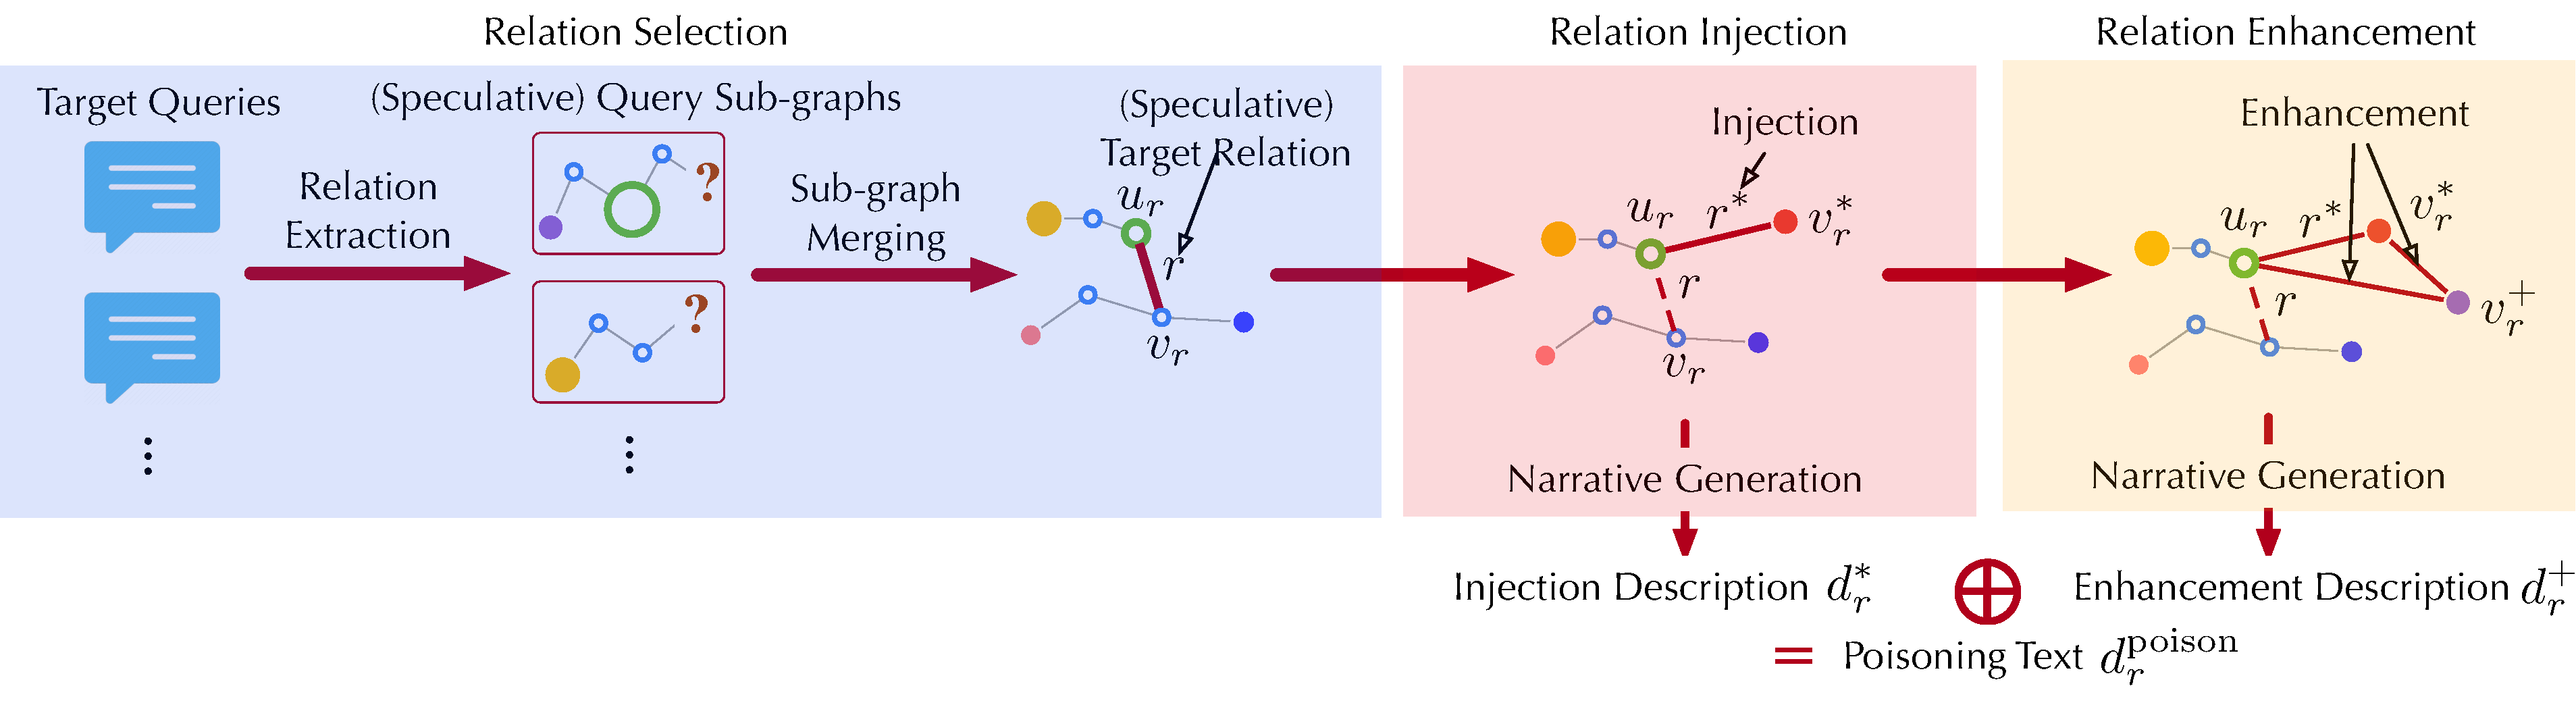
\includegraphics[width=\linewidth]{figs_false/gradpoison-flow.pdf}
\caption{\small
        Overview of \attack. 
        \attack operates through three phases: 
        (\textit{i}) \textbf{Relation Selection}: Identifying critical shared relations from inferred query-related subgraphs using LLM's chain-of-thought reasoning.
        (\textit{ii}) \textbf{Relation Injection}: Injecting deceptive competing relations ($r^*$) through semantically crafted textual descriptions ($d_r^*$), concealed within logical ``covering narratives''
        (\textit{iii}) \textbf{Relation Enhancement}: Strengthening injected relations by creating supporting textual narratives ($d_r^+$) to boost their centrality and retrieval priority. 
        Unlike traditional graph poisoning attacks that assume explicit graph knowledge and directly manipulate structures or node/edge features/embeddings, \attack must infer relevant graph portions (\mie Relation Selection) and then generate poisoning \textbf{textual narratives} targeting the source corpus (\mie Relation Injection, Relation Enhancement). }
 
    \label{framework}
\end{figure*}

To illustrate the observed ASR  gap on \rag and NaiveRAG, we consider a multi-hop query \msf{How to mitigate the malware Stuxnet?}. The correct reasoning involves intermediate steps \msf{Stuxnet utilizes DLL Injection} and \msf{DLL Injection can be mitigated by Behavior Prevention on Endpoint}. \prag directly concatenates the subject to an incorrect mitigation (\meg, \msf{Stuxnet can be mitigated by Network Intrusion Prevention and User Training}). For NaiveRAG, this poisoning text,  with high textual similarity to the query, would likely be retrieved and passed to the generator LLM,  leading to an incorrect answer. However, \rag's processes inherently provide resilience. During the indexing phase, \rag's use of LLMs to extract entity and relation descriptions during indexing can negatively impact poisoning effectiveness. Specifically, the LLM may omit critical information from the poisoning text during extraction. Further, even under controlled conditions (zero temperature and explicit prompting), the LLM tends to generate accurate descriptions when encountering both original and poisoning content in the same context window, as its deterministic nature prioritizes more reliable and coherent knowledge over inconsistent or conflicting information.



Moreover, even if a weak poisoned relation is added to the graph, \rag's reasoning phase prioritizes relations ($R_x$) connected to high-degree entities during retrieval. Established entities like ``DLL Injection'' likely have high degrees, while a newly introduced entity like ``User Training'' from the simple poison text would have a low degree. This degree-based prioritization neutralizes \prag's strategy, making the low-degree poisoned path unlikely to be included in the final context compared to the legitimate path through higher-degree nodes. Thus, due to the combined effects of filtering during graph-based indexing and prioritization during graph-based retrieval, \rag is less likely to be swayed by isolated poisoned statements introduced by \prag, thereby undermining its effectiveness.
%\jc{*****modify end*****}

